\documentclass{article}
\usepackage{amsmath}
\usepackage{graphicx} % Required for inserting images

\title{Homework 4}
\author{Keiver Pabula CHENKEHUI 3210300365}

\begin{document}
\maketitle


\section{I. Binary Representation of Decimal Numbers}

To convert \( 477 \) to binary:
\[
\begin{aligned}
477 \div 2 &= 238 \, \text{remainder} \, 1, \\
238 \div 2 &= 119 \, \text{remainder} \, 0, \\
119 \div 2 &= 59 \, \text{remainder} \, 1, \\
59 \div 2 &= 29 \, \text{remainder} \, 1, \\
29 \div 2 &= 14 \, \text{remainder} \, 1, \\
14 \div 2 &= 7 \, \text{remainder} \, 0, \\
7 \div 2 &= 3 \, \text{remainder} \, 1, \\
3 \div 2 &= 1 \, \text{remainder} \, 1, \\
1 \div 2 &= 0 \, \text{remainder} \, 1.
\end{aligned}
\]
Thus, the binary representation of \( 477 \) is:
\[
477 = 1.11011101 \times 2^8.
\]

To convert \( \frac{3}{5} = 0.6 \) to binary:
\[
\begin{aligned}
0.6 \times 2 &= 1.2 \quad \text{(integer part: 1)}, \\
0.2 \times 2 &= 0.4 \quad \text{(integer part: 0)}, \\
0.4 \times 2 &= 0.8 \quad \text{(integer part: 0)}, \\
0.8 \times 2 &= 1.6 \quad \text{(integer part: 1)}, \\
0.6 \times 2 &= 1.2 \quad \text{(repeats)}.
\end{aligned}
\]
The binary representation of \( \frac{3}{5} \) is:
\[
\frac{3}{5} = 0.100110011001\ldots.
\]
Expressed in normalized scientific notation:
\[
\frac{3}{5} = 1.00110011001\ldots \times 2^{-1}.
\]

\section{II. Floating-Point Representation}

The floating-point representation of a number \( x \) is:
\[
x = m \times \beta^e, \quad 1 \leq m < \beta,
\]
where \( m \) is the mantissa and \( \beta \) is the base.

The nearest smaller floating-point number is:
\[
x_L = (m - \Delta m) \times \beta^e,
\]
and the nearest larger floating-point number is:
\[
x_R = (m + \Delta m) \times \beta^e,
\]
where \( \Delta m \) is the smallest possible increment for the mantissa.

To compute \( x - x_L \):
\[
x - x_L = \big(m \times \beta^e\big) - \big((m - \Delta m) \times \beta^e\big) = \Delta m \times \beta^e.
\]

To compute \( x_R - x \):
\[
x_R - x = \big((m + \Delta m) \times \beta^e\big) - \big(m \times \beta^e\big) = \Delta m \times \beta^e.
\]

Since \( \Delta m = \frac{1}{\beta} \), we have:
\[
x_R - x = \beta (x - x_L).
\]

\section{III. Floating-Point Representation}

The floating-point representation of a number \( x \) is:
\[
x = m \times \beta^e, \quad 1 \leq m < \beta,
\]
where \( m \) is the mantissa and \( \beta \) is the base.

The nearest floating-point number less than \( x \) is:
\[
x_L = (m - \Delta m) \times \beta^e,
\]
where \( \Delta m \) is the smallest possible increment for the mantissa.

The nearest floating-point number greater than \( x \) is:
\[
x_R = (m + \Delta m) \times \beta^e.
\]

To compute \( x - x_L \):
\[
x - x_L = \big(m \times \beta^e\big) - \big((m - \Delta m) \times \beta^e\big) = \Delta m \times \beta^e.
\]

To compute \( x_R - x \):
\[
x_R - x = \big((m + \Delta m) \times \beta^e\big) - \big(m \times \beta^e\big) = \Delta m \times \beta^e.
\]

Since \( \Delta m = \frac{1}{\beta} \), we have:
\[
x_R - x = \beta (x - x_L).
\]

\section{IV}

From III, the binary representation of \( 35\frac{3}{5} \) is:  
\[
1.00110011001\ldots \times 2^{-1}.
\]  
The mantissa is truncated to 23 bits (including the implicit leading 1):  
\[
1.00110011001100110011001.
\]  
Mantissa increment \( 2^{-24} \):  
The nearest smaller floating-point number is:  
\[
x_L = 1.00110011001100110011 \times 2^{-1}.
\]  
The nearest larger floating-point number is:  
\[
x_R = 1.00110011001100110100 \times 2^{-1}.
\]  
The value of \( \text{fl}(x) \), the closest floating-point number, is determined by rounding up:  
\[
\text{fl}(x) = x_R.
\]  
Given \( x_R = r_L = 2^{-24} \) and \( x = x_L = 1.00110011\ldots \times 2^{-25} = \frac{3}{5} \times 2^{-24} \), we find:  
\[
x_R - x = \frac{2}{5} \times 2^{-24}.
\]  
The relative error is:  
\[
\text{Relative error} = \frac{\text{fl}(x) - x}{x} = \frac{\frac{2}{5} \times 2^{-24}}{\frac{3}{5} \times 2^{-24}} = \frac{2}{3} \times 2^{-24}.
\]

\section{V}

According to the IEEE 754 standard, if rounding is not performed but the mantissa is truncated instead, the rounding error equals the largest possible value of the truncated bits.  
For single-precision floating-point numbers, the mantissa has 23 bits. Therefore, the unit rounding error is:  
\[
\text{Unit rounding error} = 2^{-23}.
\]

\section{VI}

Let \( \cos(x) \approx 1 - \frac{x^2}{2} \) (Taylor expansion, first-order approximation).  
When \( x = \frac{1}{4} \):  
\[
\cos\left(\frac{1}{4}\right) \approx 1 - \left(\frac{1}{4}\right)^2 = 1 - \frac{1}{32}.
\]  
The number of lost digits is:  
\[
\text{Number of lost digits} = \log_2 \left( \frac{\text{absolute value of the number}}{\text{calculated result}} \right) = \log_2 \left( \frac{1}{\frac{1}{32}} \right) = \log_2 (32) = 5.
\]  
Therefore, 5 digits of precision are lost.

\section{VII}
Method 1: 
Using the trigonometric identity: 
\[ 
1 - \cos(x) = 2\sin^2\left(\frac{x}{2}\right). 
\] 
Calculating \( \sin^2\left(\frac{x}{2}\right) \) is generally more stable than directly computing \( 1 - \cos(x) \), as it avoids subtracting two nearly equal numbers. 
Method 2: 
Using the Taylor expansion: 
\[ 
\cos(x) = 1 - \frac{x^2}{2} + \frac{x^4}{24} - \cdots. 
\] 
When \( x \) is small, we can truncate after a certain term and directly compute: 
\[ 
1 - \cos(x) \approx \frac{x^2}{2}, 
\] 
to avoid the subtraction of large numbers from smaller ones. 



\section{ VIII}

\( (x - 1)^\alpha \) condition number: 
\[ 
\kappa(x) = \left| \frac{x}{f(x)} \cdot f'(x) \right| = \left| \frac{x}{(x - 1)^\alpha} \cdot \alpha (x - 1)^{\alpha - 1} \right| = \left| \frac{\alpha x}{x - 1} \right|. 
\] 
When \( x \to 1 \), \( (x - 1) \to 0 \), and the condition number becomes extremely large. 
\( \ln(x) \) condition number: 
\[ 
\kappa(x) = \left| \frac{x}{f(x)} \cdot f'(x) \right| = \left| \frac{x}{\ln(x)} \cdot \frac{1}{x} \right| = \left| \frac{1}{\ln(x)} \right|. 
\] 
When \( x \to 1 \), \( \ln(x) \to 0 \), and the condition number becomes extremely large. 
\( e^x \) condition number: 
\[ 
\kappa(x) = \left| \frac{x}{f(x)} \cdot f'(x) \right| = \left| \frac{x}{e^x} \cdot e^x \right| = |x|. 
\] 
The condition number increases as \( x \) becomes large. 
 \( \arccos(x) \) condition number: 
\[ 
\kappa(x) = \left| \frac{x}{f(x)} \cdot f'(x) \right| = \left| \frac{x}{\arccos(x)} \cdot \frac{-1}{\sqrt{1 - x^2}} \right| = \frac{x}{\arccos(x) \sqrt{1 - x^2}}. 
\] 
When \( x \to \pm 1 \), \( \sqrt{1 - x^2} \to 0 \), and the condition number becomes extremely large. 


\section{IX. Function \( f(x) = 1 - e^{-x} \)}
\subsection{1. Proof that \( \text{cond}_{f}(x) \leq 1 \):}

The derivative of \( f(x) \) is:
\[
f'(x) = e^{-x}.
\]
The condition number is defined as:
\[
\text{cond}_{f}(x) = \left| \frac{x f'(x)}{f(x)} \right| = \left| \frac{x e^{-x}}{1 - e^{-x}} \right|.
\]

For \( x \in [0, 1] \):
\begin{itemize}
    \item \( e^{-x} \in [e^{-1}, 1] \),
    \item \( 1 - e^{-x} > 0 \), and \( 1 - e^{-x} \) increases monotonically with \( x \).
\end{itemize}

Since \( x e^{-x} < 1 - e^{-x} \), we conclude:
\[
\frac{x e^{-x}}{1 - e^{-x}} \leq 1.
\]
Thus, \( \text{cond}_{f}(x) \leq 1 \) holds for all \( x \in [0, 1] \).

\subsection{2. Considering Algorithm A and Relative Error:}

Suppose Algorithm \( A \) computes \( f(x) \) and the primary source of error comes from computing the exponential function \( e^{-x} \). The relative error can be expressed as:
\[
\text{Relative error} \approx \epsilon \cdot e^{-x}.
\]

The condition number for Algorithm \( A \) is:
\[
\text{cond}_A(x) = \text{cond}_f(x) + \delta(x),
\]
where \( \delta(x) \) is an additional condition number introduced by machine error, which can typically be approximated as a constant \( \epsilon \). Therefore:
\[
\text{cond}_A(x) \approx \text{cond}_f(x) + \epsilon.
\]

\subsection{3. Visualization of \( \text{cond}_{f}(x) \) and \( \text{cond}_{A}(x) \):}
\begin{figure}[h!]
    \centering
    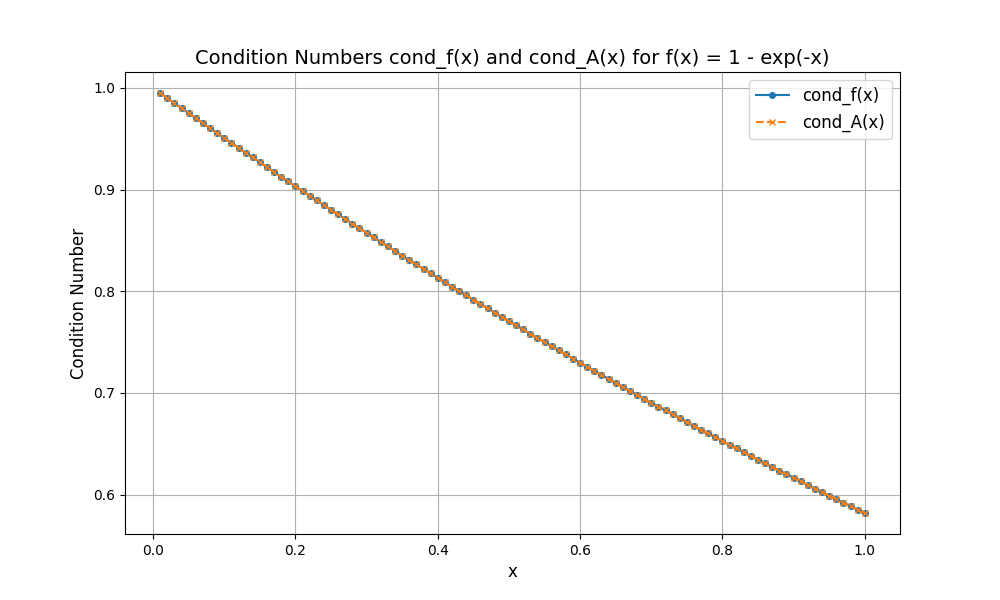
\includegraphics[width=0.7\textwidth]{Figure_1.png}
    \caption{Plot of \( \text{cond}_{f}(x) \) and \( \text{cond}_{A}(x) \) for \( f(x) = 1 - e^{-x} \).}
    \label{fig:cond_plot}
\end{figure}


\section{X. Matrix Norm and Condition Number}

The matrix norm \( \|A\|_2 \) is defined as:
\[
\|A\|_2 = \sqrt{\lambda_{\max}(A^H A)},
\]
where \( A^H \) is the conjugate transpose of \( A \), and \( \lambda_{\max}(A^H A) \) is the largest eigenvalue of \( A^H A \).

Similarly:
\[
\|A^{-1}\|_2 = \sqrt{\lambda_{\max}((A^{-1})^H A^{-1})}.
\]

The condition number is given by:
\[
\text{cond}_2(A) = \|A\|_2 \|A^{-1}\|_2.
\]

Given the singular value decomposition \( A = U \Sigma V^H \), the following holds:
\[
\lambda_i(A^H A) = \sigma_i^2,
\]
where \( \sigma_i \) are the singular values of \( A \).

Thus:
\[
\|A\|_2 = \sqrt{\lambda_{\max}(A^H A)} = \sigma_{\max},
\]
\[
\|A^{-1}\|_2 = \sqrt{\lambda_{\max}((A^{-1})^H A^{-1})} = \frac{1}{\sigma_{\min}},
\]
and:
\[
\text{cond}_2(A) = \|A\|_2 \|A^{-1}\|_2 = \frac{\sigma_{\max}}{\sigma_{\min}}.
\]

If \( A \) is a normal matrix, then \( A^H A = A A^H \), and the eigenvalues of \( A^H A \) are the squared magnitudes of the eigenvalues of \( A \). Therefore:
\[
\lambda_i(A^H A) = |\lambda_i(A)|^2,
\]
\[
\sigma_i = |\lambda_i(A)|,
\]
\[
\text{cond}_2(A) = \frac{\sigma_{\max}}{\sigma_{\min}} = \frac{|\lambda_{\max}|}{|\lambda_{\min}|}.
\]

If \( A \) is a unitary matrix, then:
\[
A^H A = I,
\]
and all eigenvalues have a magnitude of 1. Thus:
\[
|\lambda_{\max}| = |\lambda_{\min}| = 1,
\]
\[
\text{cond}_2(A) = \frac{|\lambda_{\max}|}{|\lambda_{\min}|} = 1.
\]


\section{XI. Condition Number of the Root of a Polynomial}
Consider a polynomial:
\[
q(x) = \sum_{i=0}^n a_i x^i, \quad a_n = 1, \, a_0 \neq 0
\]
Let \( r \) be a root of \( q(x) \), then:
\[
q(r) = 0 \implies \sum_{i=0}^n a_i r^i = 0.
\]

The derivative of \( q(r) \) with respect to \( a_k \) is:
\[
\frac{\partial q(r)}{\partial a_k} = r^k.
\]

Using the implicit function theorem, the derivative of \( r \) with respect to \( a_k \) is:
\[
\frac{\partial r}{\partial a_k} = -\frac{r^k}{q'(r)},
\]
where \( q'(r) \) is the derivative of \( q(x) \) with respect to \( x \):
\[
q'(r) = \sum_{i=1}^n i a_i r^{i-1}.
\]

The sensitivity vector can be written as:
\[
\mathbf{A}(r) = \left( \frac{\partial r}{\partial a_0}, \frac{\partial r}{\partial a_1}, \ldots, \frac{\partial r}{\partial a_{n-1}} \right).
\]

The condition number of the root \( r \) is:
\[
\text{cond}_f(r) = \|\mathbf{A}(r)\|_1 = \frac{1}{|q'(r)|} \cdot \sum_{i=0}^{n-1} |a_i r^i|.
\]

Since \( q(r) = 0 \), the condition number simplifies to:
\[
\text{cond}_f(r) = \frac{|r|^n}{|q'(r)|}.
\]

The Wilkinson polynomial is defined as:
\[
f(x) = \prod_{k=1}^p (x - k),
\]
where \( p \) is the degree of the polynomial, and the roots are \( r = k \).

The condition number of the root \( r \) is:
\[
\text{cond}_f(r) = \frac{r^p}{q'(r)},
\]
where:
\[
q'(r) = \prod_{k=1, k \neq r}^p (r - k).
\]

As \( p \to \infty \), the condition number grows:
\[
\text{cond}_f(r) \to \infty.
\]
This demonstrates that Wilkinson's polynomial becomes highly sensitive to coefficient changes for high-degree polynomials. As a result, numerical errors in computing roots can be significantly amplified.


\section{XII. Floating-Point Arithmetic and Rounding Error}
Consider the calculation:
\[
\frac{a}{b} = \frac{7.35}{1.47} = 5.000000.
\]
For precision \( p = 3 \), the result \( 5.000000 \) is rounded to \( 5.00 \). Since the exact result is \( 5.0 \), the actual error is zero, and the rounding error adheres to the machine arithmetic model.

Now consider the case where \( p = 3 \) and the operands are rounded before division:
\[
a = 7.35 \quad \text{is rounded to } 7.4,
\]
\[
b = 1.47 \quad \text{is rounded to } 1.5.
\]
The division yields:
\[
\frac{7.4}{1.5} = 4.93333.
\]
For \( p = 3 \), the result \( 4.93333 \) is rounded to \( 4.93 \).

The rounding error is:
\[
\text{Error} = \frac{4.93 - 5.0}{5.0} = -0.014.
\]
This error is consistent with the machine arithmetic model.



\section{XIII. Iterative Approximation and Precision Limits}
For an initial interval width of \( 1.0 \) and a target precision of \( 10^{-4} \), the error is bounded by:
\[
\frac{1.0}{2^n} < 10^{-4}.
\]
Rewriting:
\[
1.0 < 10^{-4} \cdot 2^n,
\]
\[
10^4 < 2^n.
\]
Taking the base-2 logarithm:
\[
n > \log_2(10^4) = 13.29.
\]
Thus, at least 14 iterations are required to achieve the target precision.

Using the IEEE 754 single-precision floating-point standard, the significand has 23 bits. The smallest step size is:
\[
\text{Step size} = 2^{-23} \times 2^{\text{exponent}}.
\]
For the interval \([25.5, 26.5]\):
\[
25.5 = 1.100111 \times 2^4, \quad 26.5 = 1.101001 \times 2^4.
\]
The exponent is \( 2^4 \), and the corresponding step size is:
\[
2^{-23} \times 2^4 = 2^{-19} \approx 1.91 \times 10^{-6}.
\]
If the target precision is \( 10^{-6} \) or smaller, single-precision floating-point numbers cannot meet the requirement due to the step size limitation.

\section{XIV. Matrix Structure in Cubic Splines}
In cubic spline interpolation, the coefficient matrix \( A \) is constructed based on the intervals \( h_i = x_{i+1} - x_i \) between adjacent nodes \( x_1, x_2, \ldots, x_n \). For example:
\[
A =
\begin{bmatrix}
h_1 & h_1 + h_2 & h_2 & 0 & \cdots & 0 \\
0 & h_2 & h_2 + h_3 & h_3 & \cdots & 0 \\
\vdots & \vdots & \vdots & \vdots & \ddots & \vdots \\
0 & \cdots & 0 & h_{n-2} & h_{n-2} + h_{n-1} & h_{n-1}
\end{bmatrix}.
\]

If some \( h_i \) are much smaller than other \( h_j \), the diagonal and subdiagonal elements of matrix \( A \) can have significant differences. This leads to a high condition number for \( A \).

The condition number is defined as:
\[
\kappa(A) = \|A\| \cdot \|A^{-1}\|.
\]
A high condition number indicates sensitivity to input errors, resulting in instability of the solution. For example, if the condition number of \( A \) approaches the reciprocal of the machine precision, numerical solutions may exhibit significant errors.

\section{Exercise 4.33}
\subsection{Case 1: \( b = 8.769 \times 10^4 \)}
\textbf{Align \( b \) and \( a \):}  
   \[
   b = 8.769 \times 10^4, \quad a = 1.234 \times 10^4.
   \]
\textbf{Exponent alignment:}  
   Since the magnitude of \( b \) is greater than \( a \), the result will be dominated by \( b \).
\textbf{Round to significant digits:}  
   Limit \( m_c \) to 3 significant digits:
   \[
   m_c = 8.769.
   \]
\textbf{Final result:}  
   \[
   c = 8.769 \times 10^4.
   \]


\subsection{Case 2: \( b = -5.678 \times 10^0 \)}
\textbf{Align \( b \) and \( a \):}  
   \[
   b = -5.678, \quad a = 1.234 \times 10^4.
   \]
\textbf{Result determination:}  
   Since the magnitude of \( b \) is much smaller than \( a \), the result is dominated by \( a \):
   \[
   c = a = 1.234 \times 10^4.
   \]


\subsection{Case 3: \( b = -5.678 \times 10^3 \)}
\textbf{Align \( b \) and \( a \):}  
   \[
   a = 1.234 \times 10^4, \quad b = -5.678 \times 10^3.
   \]
\textbf{Compute \( c = \text{fl}(a + b) \):}  
   Since \( b \) and \( a \) are of similar magnitude, compute:
   \[
   c = 1.234 \times 10^4 - 5.678 \times 10^3 = (1.234 - 0.5678) \times 10^4.
   \]
\textbf{Compute the result and limit significant digits:}  
   \[
   c = 0.6662 \times 10^4.
   \]
\textbf{Round to 3 significant digits:}  
   \[
   c = 0.666 \times 10^4.
   \]


\section*{Exercise 4.42}
In floating-point arithmetic, rounding errors increase as the difference in magnitude between numbers involved in the operation becomes larger. By summing positive numbers in ascending order, the loss of precision caused by small numbers being added to much larger numbers can be minimized.

\subsection{Example:}
Consider the following positive numbers:  
\[
a_1 = 10^{-3}, \quad a_2 = 10^{-2}, \quad a_3 = 10^2, \quad a_4 = 10^4.
\]
Adding the numbers directly in the given order:
\[
(a_4 + a_3) + (a_2 + a_1) = (10^4 + 10^2) + (10^{-2} + 10^{-3}).
\]
Here:
- \( 10^4 + 10^2 \) causes the loss of significant digits from \( 10^2 \),
- \( 10^{-2} + 10^{-3} \) contributes negligibly to the total sum, resulting in significant rounding errors.

Adding the numbers in ascending order:
\[
((a_1 + a_2) + a_3) + a_4 = ((10^{-3} + 10^{-2}) + 10^2) + 10^4.
\]
In this order:
- Smaller numbers are summed first, reducing their impact on larger numbers in later additions.
- The rounding errors are significantly reduced.




\section{Exercise 4.43}
The rounding error in floating-point arithmetic can be expressed as:
\[
\text{fl}(x) = x (1 + \epsilon), \quad |\epsilon| \leq \epsilon_u,
\]
where \( \epsilon_u \) is the machine precision.

Assume \( c_i = a_i b_i \):
\[
c_i = \text{fl}(a_i b_i) = a_i b_i (1 + \epsilon_i), \quad |\epsilon_i| \leq \epsilon_u.
\]

For the sum of three products:
\[
s = c_1 + c_2 + c_3.
\]
The floating-point evaluation of \( s \) is:
\[
\text{fl}(s) = (c_1 + c_2 + c_3)(1 + \epsilon_s), \quad |\epsilon_s| \leq \epsilon_u.
\]

Expanding the computation:
\[
\text{fl}(a_1 b_1 + a_2 b_2 + a_3 b_3) = \big(a_1 b_1 (1 + \epsilon_1) + a_2 b_2 (1 + \epsilon_2) + a_3 b_3 (1 + \epsilon_3)\big)(1 + \epsilon_s).
\]

For general nested operations:
\[
\text{fl}\left(\sum_i \prod_j a_{i,j}\right),
\]
each multiplication and addition introduces cumulative rounding errors.
So we can get the result is
- If the magnitudes of \( a_{i,j} \) differ significantly, the rounding error in the product \( \prod_j a_{i,j} \) becomes more pronounced.
- Compared to independent additions, nested operations amplify the propagation of rounding errors, leading to potentially larger overall inaccuracies.




\section{Exercise 4.80}

Let:
\[
\text{fl}(\sin x) = \sin x (1 + \delta_1), \quad \text{fl}(\cos x) = \cos x (1 + \delta_2),
\]
where \( |\delta_1|, |\delta_2| \leq \epsilon_u \), and \( \epsilon_u \) is the machine precision.

The function is given as:
\[
f_A(x) = \frac{\text{fl}(\sin x)}{1 + \text{fl}(\cos x)}.
\]
Substituting the expressions for \(\text{fl}(\sin x)\) and \(\text{fl}(\cos x)\), we have:
\[
f_A(x) = \frac{\sin x (1 + \delta_1)}{1 + \cos x (1 + \delta_2)} = \frac{\sin x (1 + \delta_1)}{1 + \cos x + \cos x \delta_2}.
\]
Dividing through by \(\sin x\), we get:
\[
f_A(x) = \frac{1 + \delta_1}{\frac{1}{\sin x} + \frac{\cos x}{\sin x} (1 + \delta_2)}.
\]

Since \(\frac{\cos x}{\sin x} = \cot x\), this simplifies to:
\[
f_A(x) = \frac{1 + \delta_1}{\frac{1}{\sin x} + \cot x + \cot x \delta_2}.
\]
Expanding further, we obtain:
\[
f_A(x) = f(x) \left(1 + \delta_1 - \frac{\cot x}{1 + \cos x} \delta_2\right).
\]

The relative error is approximately:
\[
\text{Relative error} \approx \left| \frac{\delta_1}{\sin x} \right| + \left| \frac{\cot x \cdot \delta_2}{1 + \cos x} \right|.
\]

The condition number is:
\[
\text{cond}_A(x) = \frac{1}{\sin x} + \frac{\cot x}{1 + \cos x}.
\]

- As \( x \to 0 \), \(\sin x \to 0\), and thus \(\frac{1}{\sin x}\) dominates. Therefore, \(\text{cond}_A(x) \to \infty\).
- When \( x \in (0, \pi/2) \), both \(\sin x\) and \(1 + \cos x\) are positive, and \(\text{cond}_A(x)\) remains bounded.

\end{document}
